\documentclass[12pt, en, eng]{mgr}

\usepackage{graphicx}
\usepackage{float}
 
\begin{document}
\engtitle{
	An application for tracking the flow of resources for Bitcoin cryptocurrency \\
}
\title{Program do śledzenia przepływu środków w sieci Bitcoin}
\date{2018}
\author{Marcin Pieczka}
\supervisor{Dr inż., Radosław Michalski, Katedre Inteligencji Obliczeniowej}
\field{Informatyka (INF)}
\maketitle

\section{Goals}
Every process of analyzing data starts with accessing the data, when analyzing Bitcoin blockchain, this first step might be the hardest one. Currently Bitcoin blockchain contains over 160GB of raw, binary data and everyone who attempts to analyze it will have to have an efficient and reliable way to work with it. Moreover users should have obvious place for creating additional API's that will be placed on the same server as the data, so that operations that for instance require big amounts of data, but return results of significantly smaller size can be implemented efficiently, gathered in one place, and blend in with the system. 
\\
\\
My goal is to create application that: 
\begin{itemize}

\item
allows fast access to blockchain data
\item
allows access over the network
\item
updates its data in constant manner
\item
provides API for Python and R
\item
is easy to install

\end{itemize}

\section{Alternative software providing similar features}
\subsubsection*{blockchain.info}

Web application blockchain.info provides free access to Bitcoin blockchain data by either website, JSON API or API's dedicated to specific languages including Python, but without support for R. Number of requests is limited.
\\
\\
Relevant API's provided by blockchain.info:
\begin{itemize}
\item
getting single block, by block hash
\item
getting single block, by hight
\item
getting multiple block headers
\item
getting single transaction, by transaction hash
\item
getting all transactions of single or multiple addresses


\end{itemize}

Most common usage scenario in analytic context is getting range of blocks, for example all block from 10.04.2017 to 20.04.2017 nonetheless blockchain.info does not provide simple way to get such data. To achieve this we would have to make thousands of requests to API providing us with single block data, and this wouldn't be fast enough.

Other and the biggest problem is the API call limit that would make working with this application impossible for larger query's

\subsubsection*{blockexplorer.com}

This web application is very similar to blockchain.info in almost every aspect, although there are some differences. Data is accessible either by website or by JSON API, but there is no Python or R API provided. Set of API's is almost identical to blockchain.info, and does not provide easy way to get multiple blocks. The main difference is that there is no official API call limit, but using tool that is not controlled by us means that such limit can appear every moment.

\subsubsection*{libbitcoin-database}

This piece of software, after installation builds in-memory database of Bitcoin blockchain, its description promises high performance. Because of almost non existing documentation it is hard to write much about it.
\\
\\
Although this software is actively developed, and at first sight it might seam like solution that fits needs of our users, there are couple problems that make use of it problematic. One drawback is coming from its biggest selling point - it, being in-memory database makes it require large amounts of RAM, probably over 160GB, witch makes it not viable for hardware that is accessible for me. Next problem is it's API, with allows connecting to this db via C/C++ library, witch would make usage in R and Python at least problematic. Another problem is lack of useful documentation, witch would make usage a really hard experience.

\subsubsection*{BitcoinDatabaseGenerator}

BitcoinDatabaseGenerator is data transfer tool that can feed SQL database with blockchain data. It was written in C\# and as its author states it is only meant to be run on Windows machines. From the documentation we know that this software should be ran every time we want to update our database. Database schema that is created after operation consists of separate tables for blocks, transactions, transaction inputs and so forth, witch would require joining those tables in multitude of usage scenarios.
\\
\\
Although you can easily connect to SQL database from both R and Python, I find working with SQL databases in such case cumbersome, it would require abstracting away relational structure of data to more object like one. 


\section{Design}

\subsection{User requirements}
\subsubsection{User stories}
As a user, I want to access blockchain data from my Python/R script so that data analysis and data accessing can be made in the same code.
\\
\\
As a user, I want the data be in a format idiomatic to Python/R so that I don't have to convert it after.
\\
\\
As a user, I want easy access to block data from range of time or block height so that I can spend my time working with the data, and not with accessing it.
\\
\\
As a user, I want the installation not to require complicated operations so that I can do it without specialized knowledge.
\\
\\
As a user, I want to be able to run this software on my linux server so that I don't have to learn new operating system to use it.
\\
\\
As a user, I want fast access to the data so that my analytic scripts will be pleasurable to work with.
\\
\\
As a future maintainer, I want to have obvious place to create my own API's on server so that my new data hungry features can be placed on the same server as data for better performance.
\\
\\
As a user, I want some goal so that some reason.
\\
\\

\subsection{System inputs and outputs}

In this section I will specify inputs and outputs of the system, witch will then help me to discover what transformation the input data will undergo, and what components are needed to provide outputs efficiently. Here I will consider only part of the project that is responsible for serving data, not the part that will be responsible for hosting future API's.

\subsubsection{Inputs}
\paragraph{Bitcoind BLK files}
The only source of bitcoin block data will be BLK files stored by full bitcoin node. Daemon process bitcoind gets blocks from neighboring nodes and stores them in data directory. The blk files in default configuration store up to 128MB of raw network format block data, and blocks are stored in order in witch they come from network. There exist multiple library's that handle parsing these files, so accessing this data will not be a problem.
\\
\\
One important thing to mention about bitcoin transactions stored in blocks is the fact that address of the sender is described as output of previous transaction.

\paragraph{Request for blocks} will be the way user communicates with the system. In this request user will specify witch blocks he wants to receive, usually it will be blocks from specified range of time, or range of height.

\subsubsection{Outputs}
\paragraph{Response on request for blocks} will contain block data in format understandable by user 


\subsection{Persistence}
The fact that transaction sender address is not stored in bitcoin blocks directly, but by reference to other transaction, creates responsibility for the system to discover this address by finding this referred transaction, and getting the address of recipient of this transaction. This of course requires substantial amount of time with should not be added to the time of user waiting for his response. 
\\
Additional thing to consider is the time needed to transform raw binary bitcoin block to widely used data format such as JSON. Knowing this we will get to the conclusion that we will need some type of persistence, and although some custom way to store this data might be better suited for our needs, I will be using a database because of constraint of time I have to build this solution.

\subsubsection{Database operations}
Lets consider database operations that will need to be fast, and those that are not so important in this regard.
\\
\\
Least important operation will be data addition, end user will not be performing these, and its performance will be my last priority.
\\
\\
Most important operation will be querying blocks, by its hash, time, and other attributes, specifically querying for range of consecutive blocks described by time frame and height range.
\\
\\
Another important operation is operation of getting transactions by hash, this will be needed for discovering address of transaction sender, and although this operation will not be in regular scenarios started by user, the number of such operations needed to discover sender address of every bitcoin transaction makes it crucial for this operation to be fast.

\subsubsection{Database choice}
At the beginning lets simplify the choice between RDBMS and NoSQL databases. Out of many NoSQL possibilities I have chosen MongoDB database based on some quick research of different NoSQL systems strengths and weaknesses.

Lets lay out some facts that will help to decide whether to use relational database, or MongoDB

\begin{itemize}
\item 
Storing blocks in RDBMS in multiple tables, for instance table for blocks and table for transactions, would require joining those tables witch is known to be slow operation.
\item 
To achieve fast querying, the data should be strongly denormalized.
\item
Storing blocks in RDBMS in one table can be impossible in most systems, due to attribute limit.
\item 
You can achieve comparable performance from MongoDB and RDBMS but MongoDB makes storing denormalized data idiomatic.
\item
MongoDB have API's for Python and R that makes data available as objects.
\end{itemize}

Based on these facts I will use as my database MongoDB. This problem seams like a perfect usage for database of such type because of its denormalized nature and native support for Python and R.


\subsubsection{Database structure}
 
Collections in MongoDB don't have structure defined upfront, if you want to have mandatory attribute in document, your application has to enforce it. Because of this, saying about database structure is not to accurate, it is easier to think about it as structure of data, and in my system the structure of data will not change a lot compared to form I will obtain it in. 

One document in MongoDB collection will be one bitcoin block, with its attributes like timestamp, hash, etc. and list of transactions, each with its own attributes like hash, inputs, outputs.

 
Indexing increases performance of querying the data and hinders the performance of operations like adding and removing data witch in this case looks like a great bargain. There might be additional memory cost associated with indexes, but this should not be a problem.

The indexes will be added to fields like block hash, time or height, adding indexing to transaction list is also a possibility and will be considered and tested. With indexes on transaction list it should be possible to quickly query for blocks containing transactions in witch given address receives or sends bitcoin, but its hard for me to speculate about this matter without thorough testing in live system.

\subsection{High level architecture}
This system will consist of separate entities, that will have their own, well defined responsibilities with will make them and overall system easy to understand and maintain.
\\
\\
System will consist of:
\begin{itemize}
\item
Bitcoin node with its data directory
\item
Database for storing processed blocks
\item
Process constantly updating database with new blocks that are gathered by bitcoin node witch I will refer to as database updater
\item
Web application ready to implement complex functionalities in
\end{itemize}

\subsubsection{Database Updater}
This component will have responsibility for parsing raw bitcoin blocks collected from BLK files, discovering transaction sender address by transaction output referred in its input, adding blocks to database and administering the database, namely adding indexes in the best moment.

Although this components performance does not add to user wait time, it adds to time needed to get to the point at witch most of the recent blocks are in the database. Because of large amount of data that needs to be processed and inserted to database, optimizations are necessary to finish initial data load in reasonable time.

The main bottleneck is discovering sender address, nowadays, one block holds about 2000 transactions, so to process one block with simplest design, database updater would have to ask the database about 2000 times for transaction for every processed block witch would lead to very poor performance. Because it would require to much memory for database updater to remember every transaction it processed, it will remember some constant number of last processed transactions.


\begin{figure}[H]
  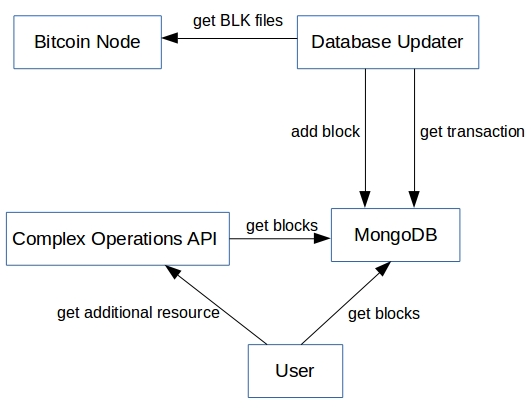
\includegraphics[width=0.8\linewidth]{component-diagram.png}
  \caption{System components and their communication}
  \label{fig:system-components-and-their-communication}
\end{figure}



\subsection{Deployment}

The main things that can be accomplished with well chosen deployment and packaging are simplicity of use and cross-platform possibilities witch can positively influence adoption rate of this solution in perspective of both usage and further open source development.

For this project I will use docker containers, witch will help in keeping components decoupled, and will make installation process not to require multiple complex steps. 

Installation process that I want to achieve should consist only of installing full bitcoin node, docker, running one custom script and setting up simple configuration (database credentials, etc.).

All the containers will be connected to the same private network, so that communications between them will be as simple to achieve as possible.

\section{Implementation}

\subsection{Install.sh}
I have decided to start with the installation script, because knowing its content will guide us by how containers are set up, how data flows between them, an will give us overview of whole system.

Install.sh starts with reading configuration from file "config.conf" in witch following things are set up:

\begin{itemize}
\item
Database credentials for administrator, and user with only read privileges
\item
Port at witch the database will be reachable
\item
Data directory of bitcoin node
\item
Directory at witch we want to store our database data
\item
Transaction cache size
\end{itemize} 

After configuration is loaded, network is being created, and building and starting of containers starts.

\subsubsection{Database container setup}
For this container I will show how such configuration looks, so that readers without experience with docker will have chance to see how it looks.

\begin{verbatim}
docker run -d \
    --name btc-blockchain-db \
    -e AUTH=yes \
    -e MONGODB_ADMIN_USER=$db_root_username \
    -e MONGODB_ADMIN_PASS=$db_root_password \
    -e MONGODB_APPLICATION_DATABASE=bitcoin \
    -p 0.0.0.0:$db_port:27017 \
    -v $database_dir:/data/db \
    --network=btcnet \
    aashreys/mongo-auth:latest
\end{verbatim}

Database container is build on "aashreys/mongo-auth:latest" docker image, witch lets us create MongoDB database with enabled authentication (by default in MongoDB authentication is not enabled).
Admin user credentials are being set, but credentials of user with read-only privilege cant be set here, because before-mentioned image does not support such action.

There are couple other things in this configuration worth noting, namely "-v" flag creates volume for container and its purpose comes from the fact that docker containers should be possible to kill without any loss, so with volume set up, when we kill our database container and run it again, the database data will not be lost.

Another important thing is setting up common network for all the containers, here it is accomplished with flag "--network". With network configured, DNS is set up automatically and it is possible to refer other containers by their names. For instance running 
\begin{verbatim}
ping btc-blockchain-db
\end{verbatim}  
from within other container connected to the same network will send messages correctly



\section{Functionality testing}

\section{Summary}

\end{document}